\newcommand{\thetm}{\begin{tikzpicture}[node distance=2.5cm,auto]
  \node(q0)[state,initial]{$q_0$};
  \node(q1)[state,right of=q0]{$q_1$};
  \node(q2)[state,right of=q1]{$q_2$};
  \node(q3)[state,right of=q2]{$q_3$};
  \node(q4)[state,above of=q3]{$q_4$};
  \node(q5)[state,accepting,below of=q0]{$q_4$};
  \path[->]       (q0) edge node{$a|\sqcup,R$} (q1)
	          (q0) edge node{$\sqcup|\sqcup,N$} (q5)
	          (q1) edge[loop above] node{$a|a,R$} ()
	          (q1) edge node{$b|b,R$} (q2)
	          (q1) edge node{$\sqcup|\sqcup,N$} (q5)
	          (q2) edge[loop below] node{$b|b,R$} ()
	          (q2) edge node{$\sqcup|\sqcup,L$} (q3)
	          (q3) edge node{$b|\sqcup,L$} (q4)
	          (q4) edge[loop above] node{$a|a,L; b|b,L$} ()
	          (q4) edge[bend right] node{$\sqcup|\sqcup,R$} (q0);
 \end{tikzpicture}}

\include{includes/common_start}
\tutnr{14}

\section{Begriffe der Informationstheorie}
\subsection{Erklärung}
\begin{frame}
	\frametitle{Shannonscher Informationsbegriff}
	\begin{itemize}
		\item Jede Information bzw. Nachricht besitzt eine Quelle
		\begin{itemize}
			\item Oft randomisiert a.k.a. Zufallsquellen
			\item Wenn alle gesendete Nachrichten unabhängig voneinander sind, ist die Quelle gedächtnislos
		\end{itemize}
		\item Es gibt immer einen Empfänger, der die Nachrichten beobachtet
		\item Je unvorhersehbarer die Nachricht, desto mehr Informationsgehalt
		\begin{itemize}
				\item Wird deshalb auch manchmal Überraschungswert genannt
		\end{itemize}
		\item Entropie ist ein Begriff für die Dichte der Informationen
	\end{itemize}
\end{frame}

\begin{frame}
	\frametitle{Etwas genauer}
	\begin{itemize}
		\item Informationsgehalt soll nicht negativ sein
		\item Ein sicheres Ergebnis (p = 1) enthält keine Information
		\item Informationen von unabhängigen Nachrichten sollen sich addieren
		\item Kleine Änderungen der Wahrscheinlichkeit $\Rightarrow$ kleine Änderung des Informationsgehalts
		\item $I(x) = -log_b(p(x)) = log_b(\frac{1}{p(x)})$ erfüllt diese Bedingungen
		\begin{itemize}
			\item Meist wird als Basis b = 2 verwendet
		\end{itemize}~\\~\\
		\item Entropie ist entsprechend definiert~\\ $H(X) = \sum\limits_{x \in X} (p(x) \cdot log_2(\frac{1}{p(x)})) = \sum\limits_{x \in X} (p(x) \cdot I(x))$
	\end{itemize}
\end{frame}

\begin{frame}
	\frametitle{Beispiele}
	\begin{itemize}
		\item Zufallsquelle 1: p(A) = $\frac{1}{2}$, p(B) = $\frac{1}{2}$
		\item I(A) = $log_2(\frac{1}{0.5}) = log_2(2) = 1$ = I(B)
		\item H(X) = $(p(A) \cdot I(A)) + (p(B) \cdot I(B)) = 0.5 + 0.5 = 1$~\\~\\~\\~\\
		\item Zufallsquelle 2: p(A) = $\frac{1}{16}$, p(B) = $\frac{15}{16}$
		\item I(A) = $log_2(\frac{1}{0.0625}) = log_2(16) = 4$
		\item I(B) = $log_2(\frac{1}{0.9375}) = log_2(\frac{16}{15}) = 0.0931\ldots$
		\item H(X) = $(p(A) \cdot I(A)) + (p(B) \cdot I(B))$~\\$= (\frac{1}{16} \cdot 4) + (\frac{15}{16} \cdot 0.0931) = \frac{1}{4} + 0.873 = 0.337$
	\end{itemize}
\end{frame}
%Explaining "Ordnung von Zeichenketten would be Bogus"

\subsection{Aufgabe B11 A1}
\begin{frame}
	\frametitle{Aufgabe B11 A1}
	\begin{enumerate}
		\item Wie gro"s sind der Informationsgehalt und die Entropie, wenn eine Quelle mit
		dem Alphabet $\{0,1\}$ nur aus dem Zeichen $0$ bestehende Folgen sendet?
		\item An einer Quelle mit $n$ Zeichen tritt jedes Zeichen gleichverteilt auf. Wie
		gro"s sind der Informationsgehalt und die Entropie eines einzelnen Zeichens?
		\item Berechnen Sie die Entropie des Wurfes eines idealen W"urfels mit 8 Seiten,
		dessen Wahrscheinlichkeit f"ur jede Seite $p = \frac{1}{8}$ ist!
		\item Was ist der Unterschied zwischen den beiden Folgen, die aus verschiedenen
		ged"achtnislosen Quellen mit der gleichen Wahrscheinlichkeit f"ur $0$ und $1$
		gesendet werden, wenn man sie unter dem Aspekt Entropie und Ordnung betrachtet?
		\begin{enumerate}
			\item ...10101010101010101010...
			\item ...01101100110111000010...
		\end{enumerate}
	\end{enumerate}
\end{frame}

\section{Huffman-Codierung}
\subsection{Erklärung}
\begin{frame}
	\frametitle{Huffman-Codierung}
	Die Huffman-Codierung ist ein Algorithmus zur verlustfreien Datenkompression.
	\begin{block}{Problemdefinition}
	\begin{itemize}
		\item Gegeben
		\begin{itemize}
			\item Ein Alphabet $A = \{a_0, a_1, ..., a_n\}$ der Größe $n$
			\item Gewichte $W = \{w_0, w_1, ..., w_n\}$ für alle $a \in A$. \\
			Meist die Wahrscheinlichkeit, dass ein Zeichen auftritt.
		\end{itemize}
		\item Gesucht
		\begin{itemize}
			\item Eine binäre Codierung für alle Zeichen aus $A$, sodass die erwartete Code-Wortlänge in Bezug auf die Gewichte minimal ist.
		\end{itemize}		
	\end{itemize}
	\end{block}
	\only<2> {
	Lässt sich sowohl auf konkrete Wörter anwenden als auch auf Quellen, von denen man weiß, wie wahrscheinlich sie welches Zeichen sendet.
	}
\end{frame}
\begin{frame}
	\frametitle{Huffman-Codierung Beispiel}
	Gegeben sei das Wort \textbf{\textcolor{red}{a}\textcolor{blue}{b}\textcolor{red}{a}\textcolor{green}{c}\textcolor{red}{a}\textcolor{blue}{b}\textcolor{red}{a}d\textcolor{red}{a}\textcolor{blue}{b}\textcolor{red}{a}\textcolor{green}{c}\textcolor{red}{a}\textcolor{blue}{b}\textcolor{red}{a}}. Wie lautet eine Huffman-Codierung? \\
	\visible<2->{
		\begin{itemize}
			\item \textcolor{red}{\#a = 8}
			\item \textcolor{blue}{\#b = 4}
			\item \textcolor{green}{\#c = 2}
			\item \textcolor{brown}{\#d = 1}
		\end{itemize}
	}
	\only<3>{
		\begin{center}
			\includegraphics[scale=0.4]{images/Huffman}
		\end{center}
	}
\end{frame}
\subsection{Aufgabe B11 A3}
\begin{frame}
	\frametitle{Aufgabe B11 A3}
	Gegeben sei eine Quelle mit Alphabet $\{A,B,C,D\}$ und mit den folgenden
	Wahrscheinlichkeiten:\\
	$P(A)=\frac{1}{2}, P(B)=\frac{1}{4}, P(C)=\frac{1}{8}, P(D)=\frac{1}{8}$
	\begin{itemize}
	\only<1>{
		\item Berechnen Sie die Entropie der Quelle!
		\item Erstellen Sie eine entsprechende Huffman-Codierung!
		\item Was ist die mittlere Codewortl"ange? Gibt es einen Zusammenhang zur Entropie?
		}
		\only<2>{
		\item Gegeben sei der folgende Huffman-Baum:
		\begin{center}
			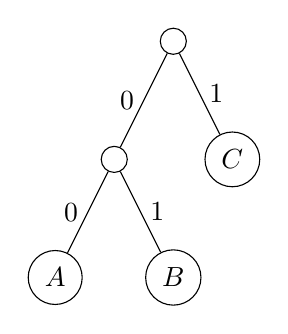
\begin{tikzpicture}
				\node[circle,draw]{}
				child{
				  node[circle,draw]{}
				  child{
				    node[circle,draw]{$A$}
				    edge from parent
				    node[left]{\textbf{$0$}}
				  }
				  child{
				    node[circle,draw]{$B$}
				    edge from parent
				    node[right]{\textbf{$1$}}
				  }
				  edge from parent
				  node[left]{\textbf{$0$}}
				}
				child{
				  node[circle,draw]{$C$}
				  edge from parent
				  node[right]{\textbf{$1$}}
				};
			\end{tikzpicture}
		\end{center}
		Dekodieren Sie $011011101100101011$! Ist der Huffman-Code geeignet?
		}
	\end{itemize}
\end{frame}

\section{Multiple Choice}
\subsection{Multiple Choice}
\begin{frame}
	\frametitle{Multiple Choice}
	\begin{center}
	\only<1>{
		Das Hamilton-Kreis Problem ist NP-vollständig
	}
	\only<2>{
		In der Klasse NP liegen nicht-entscheidbare Probleme
	}
	\only<3>{
		Das Vertex-Cover Problem ist NP-vollständig
	}
	\only<4>{
		Semi-entscheidbare Sprachen sind unter Komplementbildung
abgeschlossen
	}
	\only<5>{
		Nichtdeterministische endliche Automaten sind echt mächtiger als
deterministische
	}
	\only<6>{
		Zu jeder CH-2-Sprache gibt es eine CH-1-Grammatik
	}
	\only<7>{
		Um zu zeigen, dass ein Problem $\Pi$ NP-vollständig ist, genügt es, ein NP-schweres Problem auf $\Pi$ zu reduzieren.
	}
	\only<8>{
		Das Travelman Salesmen Problem ist NP-vollständig
	}
	\only<9>{
		N-SAT ist immer NP-vollständig
	}
	\only<10>{
		Deterministische Kellerautomaten erkennen Chomsky-2
	}
	\only<11>{
		$ NP \neq co-NP \implies P \neq NP $
	}
	\end{center}
\end{frame}

\section{Schluss}
\subsection{Schluss}
\begin{frame}
	\frametitle{Bis zum nächsten Mal!}
    \begin{center}
        \includegraphics[height=0.85\textheight]{images/password_strength.png}
    \end{center}
\end{frame}

\include{includes/common_end}
